% Search for all the places that say "PUT SOMETHING HERE".

\documentclass[11pt]{article}
\usepackage{amsmath,textcomp,fancyvrb,pdfpages, amssymb,geometry,graphicx,enumerate,bm,hyperref}
\graphicspath{ {images/} }

\title{CS189--FALL 2015 --- Homework 6 Write up}
\author{ZUBO GU, SID 25500921, gu.zubo@berkeley.edu}
\markboth{}{}
\pagestyle{myheadings}
\date{}

\begin{document}
\maketitle

\section*{Problem 1}
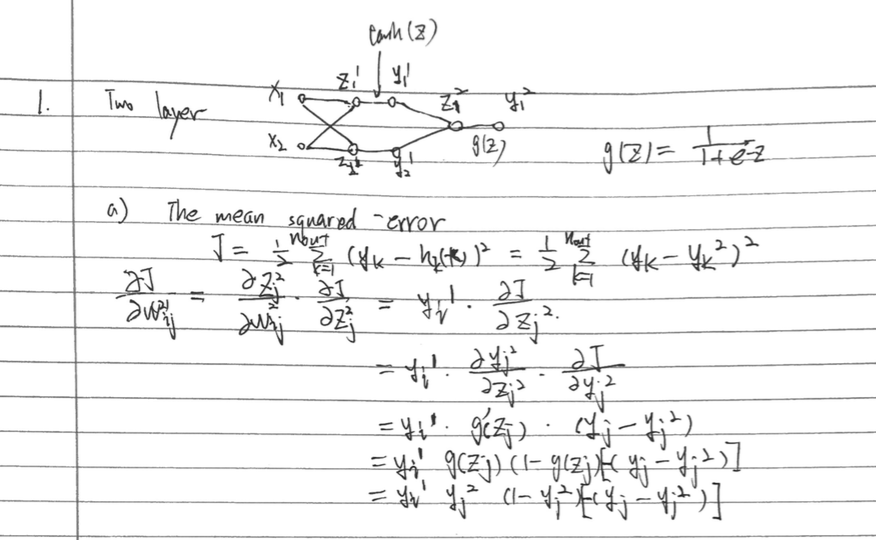
\includegraphics[scale = 0.5]{1.png}

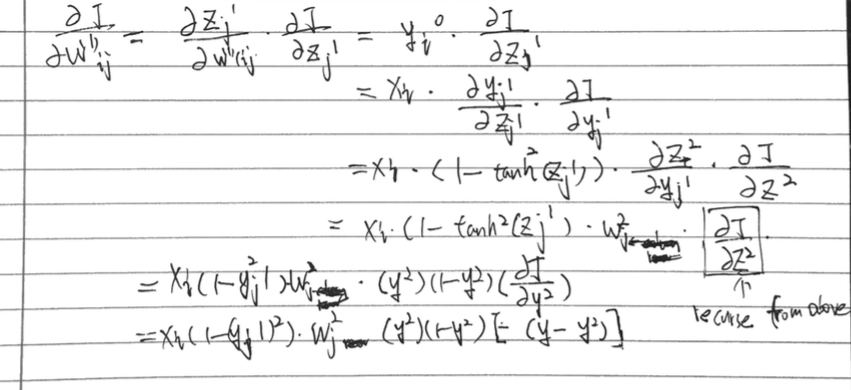
\includegraphics[scale = 0.5]{2.png}

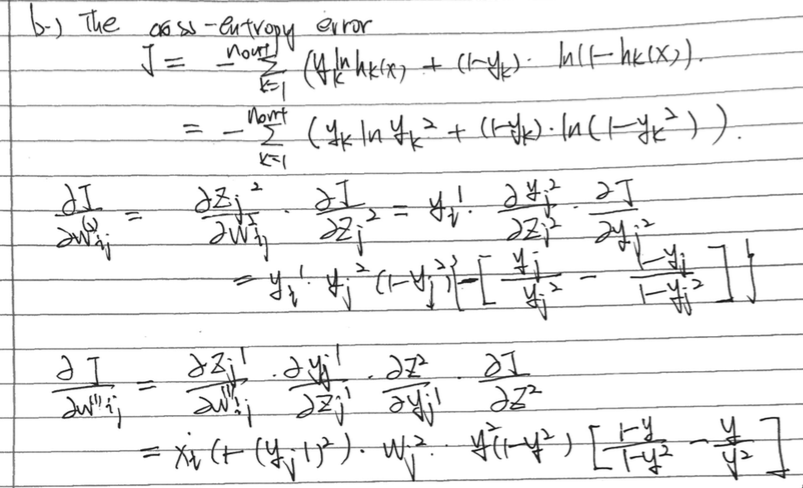
\includegraphics[scale = 0.5]{3.png}

\section*{Problem 2}
The best kaggle score is 0.94840.

\begin{itemize}
\item[1.]
I have learning rate $\eta$ = 2 by using mean squared error loss function.

The training will stop when I can't see improvement in 1000000 iteration.

The initial W1 and W2 are two matrices with dimension 785 x 200 and 201 x 10. All entry are random with mean 0 variance 1.

\item[2.]
training accuracy 0.99322
validationset accuracy 0.9552

\item[3.]
10h

\item[4.]

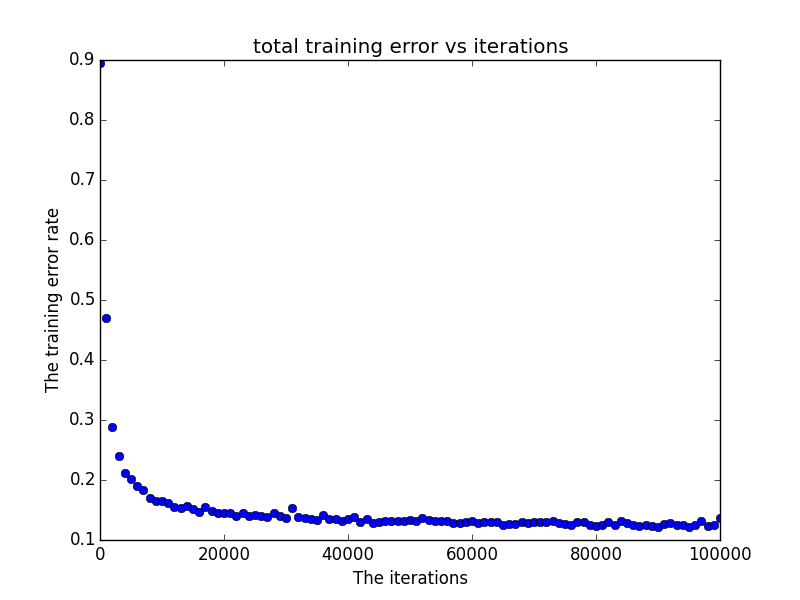
\includegraphics[scale = 0.5]{4.png}

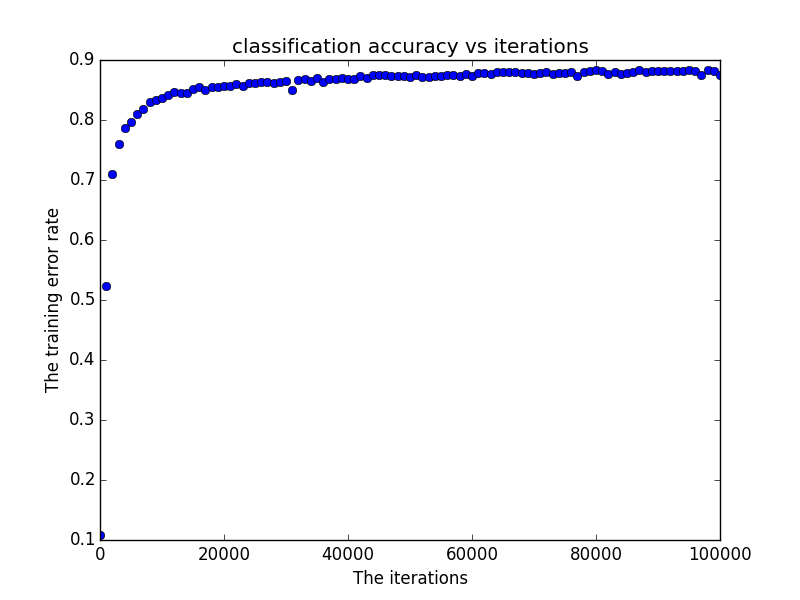
\includegraphics[scale = 0.5]{5.png}

\item[5.]
The mean squared error loss function is more fit for the training data whose training accuracy is much higher than validation set accuracy. The cross entropy is not that much over fit.
The cross entropy is better in performance.


\end{itemize}


\newpage
\section*{Code}
\VerbatimInput[baselinestretch=1,fontsize=\footnotesize,numbers=left]{hw6.py}


\end{document}


